\documentclass[a4paper]{article}

\usepackage[pages=all, color=black, position={current page.south}, placement=bottom, scale=1, opacity=1, vshift=5mm]{background}
\SetBgContents{
	\tt Análisis de algoritmos 2022-1
}      % copyright

\usepackage[margin=1in]{geometry} % full-width

% AMS Packages
\usepackage{amsmath}
\usepackage{amsthm}
\usepackage{amssymb}
\usepackage{graphicx}
\usepackage{enumitem}
\usepackage{algorithm, algpseudocode}
% Unicode
\usepackage[utf8]{inputenc}
\usepackage{hyperref}

\usepackage{outlines}
\hypersetup{
	unicode,
%	colorlinks,
%	breaklinks,
%	urlcolor=cyan, 
%	linkcolor=blue,
	pdfauthor={Author One, Author Two, Author Three},
	pdftitle={A simple article template},
	pdfsubject={A simple article template},
	pdfkeywords={article, template, simple},
	pdfproducer={LaTeX},
	pdfcreator={pdflatex}
}

% Vietnamese
%\usepackage{vntex}

% Natbib
\usepackage[sort&compress,numbers,square]{natbib}
\bibliographystyle{mplainnat}

% Theorem, Lemma, etc
\theoremstyle{plain}
\newtheorem{theorem}{Theorem}
\newtheorem{corollary}[theorem]{Corollary}
\newtheorem{lemma}[theorem]{Lemma}
\newtheorem{claim}{Claim}[theorem]
\newtheorem{axiom}[theorem]{Axiom}
\newtheorem{conjecture}[theorem]{Conjecture}
\newtheorem{fact}[theorem]{Fact}
\newtheorem{hypothesis}[theorem]{Hypothesis}
\newtheorem{assumption}[theorem]{Assumption}
\newtheorem{proposition}[theorem]{Proposition}
\newtheorem{criterion}[theorem]{Criterion}
\theoremstyle{definition}
\newtheorem{definition}[theorem]{Definition}
\newtheorem{example}[theorem]{Example}
\newtheorem{remark}[theorem]{Remark}
\newtheorem{problem}[theorem]{Problem}
\newtheorem{principle}[theorem]{Principle}

\usepackage{graphicx, color}
\graphicspath{{fig/}}

%\usepackage[linesnumbered,ruled,vlined,commentsnumbered]{algorithm2e} % use algorithm2e for typesetting algorithms
\usepackage{algorithm, algpseudocode} % use algorithm and algorithmicx for typesetting algorithms
\usepackage{mathrsfs} % for \mathscr command

\usepackage{lipsum}
\usepackage{listings}

% Author info
\title{Análisis de algoritmos : Proyecto final}
\author{Fabián Rojas$^1$ \and Julián Tarazona$^1$}


\date{
	$^1$Pontificia Universidad Javeriana \\ \texttt{\{fabian-rojasm, jdtarazona\}@javeriana.edu.co}\\%
	\today
}

\begin{document}

\maketitle
    \section{Resumen}
	    \label{sec:def}
	    \hspace{1mm}
	    En este documento se presenta el análisis, diseño e implementación de un algoritmo para un jugador automático para el juego de Taquin o sliding-puzzle haciendo uso de arboles, búsqueda en profundidad y de una función heurística.
	    
	\section{Análisis y diseño}
	    \label{sec:def}
	    \subsection{Análisis}
	    
	    El Taquin o Sliding puzzle, son rompecabezas que desafían al jugador a deslizar las piezas de forma que este pueda establecer un patrón objetivo. Las piezas para mover pueden ser patrones de números, letras, colores, etc. Los tableros más conocidos de este juego son los de tamaño 3x3 o 4x4.[1]\newline
	    
	    El problema del jugador automático radica en ordenar los elementos de un tablero de tamaño nxn de forma que en cada una de sus filas los elementos queden ordenados de forma ascendente, tal como se muestra en la figura 1. Para el desarrollo de este algoritmo, los elementos del tablero se definen como $C =\left\langle c \in \mathbb{N};1 \le c \le n*n \right\rangle$ donde n es el tamaño del tablero.
	    
	    \begin{figure}[h]
        
        \centering
        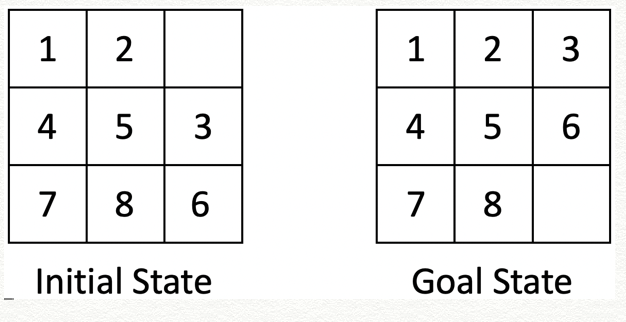
\includegraphics[scale=0.4]{phpPup4AX.png}
        \caption{Ejemplo de un juego de Taquin en tablero de 3x3}
        \end{figure}
	    
	    El jugador automático solo puede mover las casillas que tengan a su lado un espacio vacío, pero no en sus diagonales, limitando el movimiento de las piezas en 4 posibles opciones: derecha, izquierda, arriba y abajo.\newline
	    
	    Para que el jugador automático pueda decidir que movimiento realizar que lo acerquen a la victoria se hará uso de árboles, búsqueda en profundidad y de una función heurística. Para la estructura del árbol se define que los nodos estarán constituidos por los siguientes elementos:
	    \newline
	    \begin{itemize}
	       \item El tablero de Taquin.
	       \item El movimiento que se realizo para llegar al estado actual del tablero.
	       \item El estado del tablero anterior.
	       \item Todos los posibles movimientos que se pueden realizar con el estado del tablero actual.
	    \end{itemize}
	    
	    El árbol tendrá un máximo de 4 niveles para limitar el espacio en memoria ocupado. En el cuarto nivel del árbol se encontrarán los nodos hoja que contarán con su respectivo cálculo de la heurística, cabe aclarar que en los niveles superiores no se realiza el cálculo de dicha función.\newline
	    
	    Para la función heurística se calcula la distancia a la cual se encuentra cada pieza de su posición objetivo, se muestra un ejemplo en la figura 2. Cuando ya se tengan todos estos valores, se procede a realizar la sumatoria de los valores que dará como resultado el valor de la función heurística.\newline
	    
	    \begin{figure}[h]
        
        \centering
        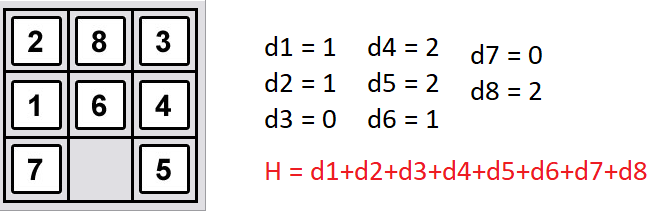
\includegraphics[scale=0.4]{figura2.png}
        \caption{Ejemplo de heuristica en un tablero de 3x3}
        \end{figure}
	    
	    Al tener el árbol construido con todos sus respectivos nodos, se realiza una búsqueda en profundidad de los nodos hojas, al encontrar estos nodos se toma aquel que tenga el valor de la función heurística más bajo, de este se realiza backtracking con el fin de obtener los movimientos que se realizaron para llegar a ese nodo hoja. Este proceso se repite hasta que se encuentre el patrón ganador del juego.\newline
	    
	    \subsection{Diseño}
	    \hspace{1cm}
	    \begin{outline}[enumerate]
	
	    \1 \textbf{Entradas:}
	    	
	        \begin{itemize}
	            \item Una matriz cuadrada de tamaño n dentro de la cual hay un conjunto de elementos C definidos como $C =\left\langle c \in \mathbb{N};1 \le c \le n*n \right\rangle$
	    
	        \end{itemize}
	
	    
	    \1 \textbf{Salidas:} 
	       
	        \begin{itemize}
	            \item Una lista de acciones que permiten ganar el juego.
	            
	        \end{itemize}
	        
	     \end{outline}
	
	\section{Algoritmos}
	    
	    \begin{algorithm}[H]
        \begin{algorithmic}[1]
        
        \Procedure{jugar}{$tablero$}
        
            \State$pila\_de\_movimientos \leftarrow \emptyset$
            \State$arbol \leftarrow Nodo(tablero)$
        
              \While{$\lnot seHaGanado()$}
            
                \State$extenderArbol(arbol, 2)$
                \State$nodos4toNivel \leftarrow \emptyset$
                \State$buscarHijos4toNivel(arbol, nodos4toNivel)$
                \State$min\_heuristica \leftarrow -\infty$
                \State $nodoEscogido \leftarrow \infty$
                \For {$hijo \in nodos4toNivel$}
                    \If{$hijo.heuristica < minHeuristica$}
                        \State $nodoEscogido \leftarrow hijo$
                    \EndIf
                \EndFor
                \State $arbol \leftarrow nodoEscogido$
            \EndWhile
            \State crearPilaDeMovimientos($nodoEscogido, pila\_de\_movimientos$)
          
            \State $Reverse( pila\_de\_movimientos )$  
        
            \State\Return $pila\_de\_movimientos$
        \EndProcedure
        
        \end{algorithmic}
        
        \caption{Jugador automático}
        \end{algorithm}
        
        En el algoritmo 1 se muestra el procedimiento que realiza el jugador automático para jugar Taquin. Comienza tomando el estado inicial del tablero y procede a crear el árbol con todas las posibles jugadas en la función extenderArbol, cuando se finaliza la creación del árbol se procede a buscar los nodos hojas del cuarto nivel que tendrán los valores de la función heurística para cada estado del tablero. Al conocer todos los nodos hoja se busca cual de estos tiene el valor de la heurística mas bajo y partir de este crea la pila de movimientos realizando el backtracking hasta el nodo raíz. Por ultimo la función reverse invierte el orden de la pila de movimientos.
        
        \begin{algorithm}[H]
        \begin{algorithmic}[1]
        
        \Procedure{Heuristica}{$tablero$}
            \State $H \leftarrow 0$
            \For {$i \leftarrow 1 \textbf{to} |tablero| * |tablero|$}
                \State $PosCasillaActual \leftarrow coordenadas (fila,columna)$ de i
                \State $PosCasillaGanador \leftarrow coordenadas (fila,columna)$ de i
                \State
                \State $DistFila \leftarrow |PosCasillaGanador[0] - PosCasillaActual[0]|$
                \State $DistColumna \leftarrow |PosCasillaGanador[1] - PosCasillaActual[1]|$
                \State
                \State $H \leftarrow H + (DistFila + DistColumna)$
            \EndFor
            \State \Return $H$
        \EndProcedure
        
        \end{algorithmic}
        
        \caption{Calculo de heuristica}
        \end{algorithm}
        
        \begin{algorithm}[H]
        \begin{algorithmic}[1]
        
        \Procedure{extenderArbol}{$nodo, nivel$}
            \State $movimientos \leftarrow getMovimientosPosibles()$
            \If{$nivel = 4$}
                \For{$movimiento \in movimientos$}
                    \State$hijo \leftarrow hacerMovimiento(movimiento, nodo.tablero)$
                    \If{$\lnot nodo.padre.tablero = hijo$}
                        \State $nodo.hijos.add( Nodo( hijo, movimiento, nodo, heuristica(hijo) ) )$
                    \EndIf
                \EndFor
                
            \Else
                \For{$movimiento \in movimientos$}
                    \State$hijo \leftarrow hacerMovimiento(movimiento, nodo.tablero)$
                    \If{$\lnot nodo.padre = \emptyset$}
                        \If{$\lnot nodo.padre.tablero = hijo$}
                            \State $nuevoNodo \leftarrow Nodo( hijo, movimiento, nodo, \emptyset )$
                            \State $nodo.hijos.add( nuevoNodo )$
                            \State $extenderArbol(nuevoNodo, nivel + 1)$
                        \EndIf
                    \Else
                        \State $nuevoNodo \leftarrow Nodo( hijo, movimiento, nodo, \emptyset )$
                        \State $nodo.hijos.add( nuevoNodo )$
                        \State $extenderArbol(nuevoNodo, nivel + 1)$
                    \EndIf
                \EndFor
            \EndIf
        \EndProcedure
        
        \end{algorithmic}
        
        \caption{Extensión del árbol}
        \end{algorithm}
	    En el algoritmo 3 se muestra el procedimiento para crear el árbol de posibles jugadas. Se comienza creando una lista con los movimientos que se pueden ejecutar, para validar que estos son posibles se utiliza la función getMovimientosPosibles que verifica según la posición de la casilla vacía que movimientos son prohibidos y los remueve de la lista de movimientos. Continua con la parte recursiva del algoritmo, en esta sección se crean tableros a partir de la lista de movimientos y dichos tableros se convierten en nodos para luego ser incluidos en la lista de posibles movimientos del nodo actual. Cuando se llega al nivel 4 del árbol se repite el procedimiento anterior pero con la diferencia de que los tableros hijos se les incluye el valor de su función heurística.
	    
    \section{Implementación}
    \hspace{1mm}
    Anexo a este documento se encuentra el algoritmo del juego Taquin en el lenguaje Python. 
	
    \section{Complejidad}
    \hspace{1mm}
    Para el calculo de la complejidad de este algoritmo se tuvo en cuenta la complejidad de crear el árbol de posibles jugadas, esto tendría un resultado de $O(n^3)$ siendo n la cantidad de hijos que puede tener un nodo (máximo 4 hijos ya que son solo 4 movimientos) y que el arbol tiene 3 niveles sin contar la raiz del arbol. La búsqueda en profundidad que se debe realizar para hallar los nodos hoja del árbol. Dicha complejidad sería un valor de O(v) siendo v la cantidad de nodos del arbol. Por lo tanto la complejidad del algoritmo seria $O(v*n^3)$.
  
    \section{Resultados obtenidos}
    \hspace{1mm}
    Tras realizar la implementación del algoritmo se pudo evidenciar que este no lograba llegar al estado objetivo del juego, por lo que se piensa que la razón de esto sea por la función heurística, la cual no tiene en cuenta que, para llevar a ciertas casillas a sus posiciones, se debe mover otras que ya estaban en su posición objetivo. Esto hace que el algoritmo se mantenga en un ciclo infinito.
    \section{Bibliografía}
	\hspace{1cm}
	
	[1] “Sliding puzzle”, Wikipedia. el 29 de mayo de 2022. Consultado: el 31 de mayo de 2022. [En línea]. Disponible en: https://en.wikipedia.org/w/index.php?title=Sliding_puzzle&oldid=1090507304
	
	
	
\end{document}